\documentclass[13pt]{article}
\usepackage{ucs}
\usepackage[utf8x]{inputenc}
\usepackage[russian]{babel}
\usepackage[pdftex]{graphicx}
\usepackage{multirow}
\title{Лабораторная работа №7\\Определение ускорения свободного падения}
\author{Хафизов Фанис}
\begin{document}
	\begin{figure}
		\centering
		
\includegraphics[width=0.3\linewidth]{logo}
	\end{figure}
	\maketitle
	\newpage
	\section{Цель работы}
	Целью лабораторной работы является изучение процессов и параметров сво-
	бодных колебаний и параметров математического и физического маятников.
	\section{Схема установки}
	\begin{figure}[h]
		\centering
		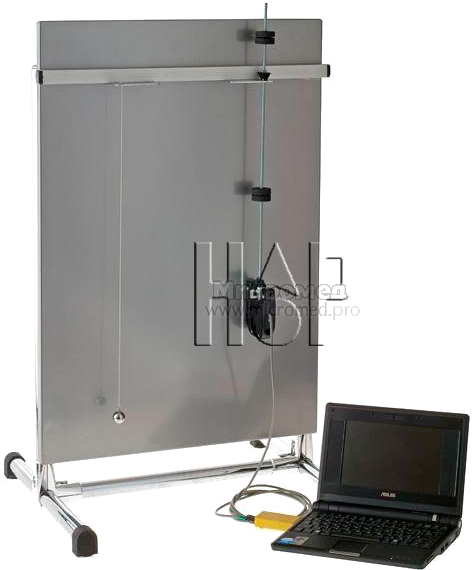
\includegraphics[scale=0.3]{image1}
		\caption{Схема установки}
	\end{figure}
	Лабораторный стенд включает в себя физическую модель математического маятника, физический (оборотный) маятник и оптоэлектрический датчик.
	К приборам и принадлежностям относятся также компьютер с необходимым
	программным обеспечением, соединетельный кабель для подключения оптоэлектрического датчика к компьютеру, измерительная линейка.
	\section{Порядок действий}
	1)Я измерил расстояние от подвеса до середины шарика математического маятника и расстояние между призмами оборотного маятника.\\
	2)Собрал лабораторную установку и закрепил оптоэлектрический датчик под шариком.\\
	3)Отвел шарик от положения равновесия и запустил измерения на компьютере. Затем отпустил шарик и подождал пока шарик пересечет датчик 10 раз, после чего остановил измерения. Выбрал по 5 пар четных и нечетных границ импульсов перекрытий и занес данные в таблицу. Повторил эксперимент еще 4 раза.\\
	4)Повторил пункты 2,3 для оборотного маятника.
	\section{Таблицы данных и графики}
	\begin{figure}[h]
		\centering
		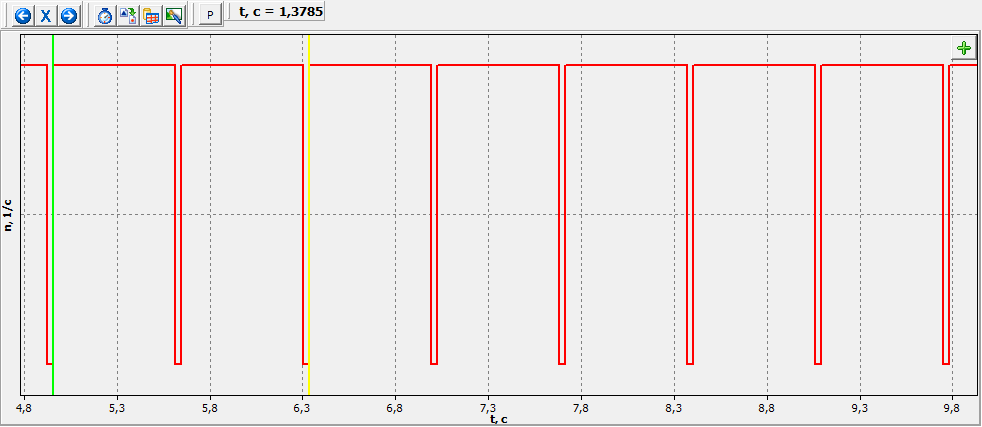
\includegraphics[scale=1.5]{graph1}
		\caption{График перекрытия датчика для математического маятника}
	\end{figure}
		\begin{figure}[h]
		\centering
		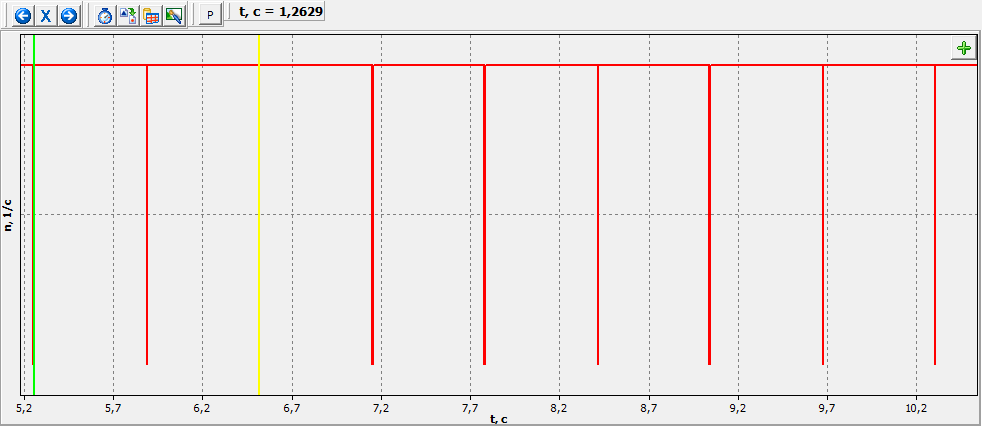
\includegraphics[scale=1.5]{graph2}
		\caption{График перекрытия датчика для физического маятника}
	\end{figure}
	\begin{table}[h]
		\caption{Длины маятников}
		\centering
		\begin{tabular}{|c|c|}
			\hline
			$l$, мм&$l_0$, мм\\
			\hline
			470$\pm$2&395$\pm$1\\
			\hline
		\end{tabular}
	\end{table}
	
	\begin{table}[h]
		\caption{Таблица 2}
		\centering
		\begin{tabular}{|c|c|c|c|c|c|c|}
			\hline
			i&Период&Ускорение&Среднее&Период&Ускорение&Среднее\\
			&математи-&свободного&ускорение&математи-&свободного&ускорение\\
			&ческого&падения&свободного&ческого&падения&свободного\\
			&маятника&$g_{mi}$, м/с$^2$&падения&маятника&$g_{phi}$, м/с$^2$&падения\\
			&$T_{mi}$, c&&$\overline{g}_m$, м/с$^2$&$T_{phi}$, с&&$\overline{g}_{phi}$, м/с$^2$\\
			\hline
			1&1,3792&9,754&\multirow{5}*{9,768}&1,2597&9,827&\multirow{5}{*}{9,813}\\
			\cline{1-3}
			\cline{5-6}
			2&1,3774&9,780&&1,2628&9,779&\\
			\cline{1-3}
			\cline{5-6}
			3&1,3767&9,790&&1,2612&9,804&\\
			\cline{1-3}
			\cline{5-6}
			4&1,3797&9,747&&1,2592&9,835&\\
			\cline{1-3}
			\cline{5-6}
			5&1,3783&9,767&&1,2600&9,822&\\
			\hline
			
		\end{tabular}
	\end{table}
	\newpage
	\section{Расчеты}
	$g_{mi}=\frac{4\pi^2l}{T_{mi}^2}$\\
	$g_{phi}=\frac{4\pi^2l_0}{T_{phi}^2}$\\
	$\overline{g}_m=\frac{\sum\limits_{i=1}^5g_{mi}}{5}$\\
	$\overline{g}_{ph}=\frac{\sum\limits_{i=1}^5g_{phi}}{5}$\\
	Оценка погрешностей:\\
	1)$\Delta g_m=2\cdot\sigma_{gm}+\overline{g}_m\cdot\varepsilon_{l}$\\
	$\sigma_{gm}=\sqrt{\frac{\sum\limits_{i=1}^{5}(g_{mi}-\overline{g}_m)^2}{5}}=0,015$ м/с$^2$\\
	$\varepsilon_l=\frac{\Delta l}{l}=0,004$\\
	$\Delta g_m=2\cdot0,015+9,768\cdot0,004=0,069$ м/с$^2$\\
	$\varepsilon_{gm}=\frac{\Delta g_m}{\overline{g}_m}=\frac{0,069}{9,768}=0,007=0,7\%$\\\\
	2)$\Delta g_{ph}=2\cdot\sigma_{gph}+\overline{g}_{ph}\cdot\varepsilon_{l0}$\\
	$\sigma_{gph}=\sqrt{\frac{\sum\limits_{i=1}^{5}(g_{phi}-\overline{g}_{ph})^2}{5}}=0,02$ м/с$^2$\\
	$\varepsilon_{l0}=\frac{\Delta l_0}{l_0}=0,0025$\\
	$\Delta g_{ph}=2\cdot0,02+9,813\cdot0,0025=0,065$ м/с$^2$\\
	$\varepsilon_{gph}=\frac{\Delta g_{ph}}{\overline{g}_{ph}}=\frac{0,065}{9,813}=0,007=0,7\%$
	\section{Результаты}
	$g_m=\overline{g}_m\pm\Delta g_m=(9,768\pm0,069)$ м/с$^2$\\
	$g_{ph}=\overline{g}_{ph}\pm\Delta g_{ph}=(9,813\pm0,065)$ м/с$^2$\\
	\section{Вывод}
	В обоих случаях я получил точный результат. В первом и втором экспериментах относительная погрешность составляет 0,7\%, причем случайная и приборная погрешности сопоставимы. Для увеличения точности результата можно было бы увеличить массу маятников.
\end{document}